\chapter{Supplementary Material for Chapter~\ref{ch:kai0}}\label{app:kai0}

This appendix provides supplementary material for Chapter~\ref{ch:kai0}. Section~\ref{kai0:app:questions} discusses motivating questions that offer alternative perspectives on the work. Section~\ref{kai0:app:related} reviews further related work on robustness from reinforcement learning and on control methods. Section~\ref{kai0:app:method} gives implementation details of the three components, and Section~\ref{kai0:app:exp} describes the experimental protocols, including hyper-parameters, scoring, hardware and training. Section~\ref{kai0:app:ablation} reports additional ablations, Section~\ref{kai0:app:failure} analyses failure cases, and Section~\ref{kai0:app:license} states the licences of the released data and code.

%-------------------------------------------------------------------------------
\section{Motivating Questions}\label{kai0:app:questions}

This section collects questions that readers may raise, together with questions that reach beyond the scope of this work.

\paragraph{Q1. What is the relationship between Stage Advantage and reinforcement learning?}
Stage Advantage follows the paradigm of advantage-weighted regression (AWR)~\cite{peng2019awr}, which can be seen as offline reinforcement learning (RL)~\cite{sutton1998reinforcement} in which the Monte Carlo reward is computed directly from data. Because such learned rewards show a large variance, advantage-weighted diffusion policies~\cite{frans2025diffusion}, and their large-scale validation in $\pi^{*}_{0.6}$~\cite{amin2026pistar06}, instead parameterise a Q-network learned from the demonstration data. Stage Advantage follows the paradigm of $\pi^{*}_{0.6}$ while comparing temporal smoothness and downstream policy performance separately. The exact objective or conditioning using its optimality signal remains to be verified (Section~\ref{kai0:app:sa}).

\paragraph{Q2. Why not use online RL such as PPO?}
PPO~\cite{schulman2017PPO} and its adaptations to diffusion-based policies, such as DSRL~\cite{wagenmaker2025dsrl}, represent another trend in RL, referred to as online RL, which learns directly from interaction with the environment. These methods are fundamentally limited by sample inefficiency in the real world. Unlike in simulation, scaling physical experiments is constrained by the prohibitive costs of parallelisation and resetting, which constitute a major bottleneck. In contrast, AWR~\cite{peng2019awr} incurs only a marginal labelling cost to bias the learning objective towards actions that make high progress, and it thereby maximises the utility of both human demonstrations and policy rollouts.

\paragraph{Q3. Why choose $\pi_{0.5}$ as the primary baseline?}
The source reports preliminary adaptation attempts with X-VLA~\cite{zheng2025xvla}, GO-1~\cite{bu2025agibot_iros}, UniVLA~\cite{bu2025univla} and OpenVLA~\cite{kim2024openvla}, with negligible success in the tested settings. These observations motivated using $\pi_0$ and $\pi_{0.5}$ for the main comparisons. Their complete configurations, tuning budgets and trial outcomes, including the DexVLA comparison mentioned in the main text, are not supplied; the preliminary screen is not a controlled ranking of foundation models.

\paragraph{Q4. How can an informative advantage be defined and designed?}
This is a critical direction for future work. Naive behaviour cloning treats all demonstrated actions equally, although many of them lack explicit utility. Training on such non-informative segments can bias the policy towards meaningless behaviours, resulting in local optima in which the robot repeats actions without making progress. Advantage weighting offers a mechanism to filter out these behaviours by emphasising actions that yield high returns. The current formulation, however, relies on a heuristic proxy, namely using temporal progress to label the advantage, which assumes that task completion is strictly monotonic. A more robust solution would replace this heuristic with an unsupervised advantage estimator capable of distinguishing truly instrumental actions from noise, independently of temporal linearity.

\paragraph{Q5. How can good robot data be defined?}
Empirically, we observed that data quality is a governing factor in policy performance, accounting for fluctuations in success rate between 20\% and 60\% under identical settings. This is an observation reported by the authors, not a result supported by a controlled experiment in this thesis. We also observe a ``masking effect'': some algorithmic improvements yield substantial gains on low-quality data but saturate or vanish when the policy is trained on high-quality demonstrations. Data quality appears to be central to the current trend of imitation learning, yet little of the literature discusses it seriously. To address this overlooked variable, we state \emph{replay-ability} as one of the most important principles of data validity. A trajectory is replay-able if its open-loop re-execution from a similar initial state leads to task completion, or at least to significant progress. This criterion not only filters out corrupted demonstrations but also serves as a diagnostic tool that exposes systematic hardware inconsistencies between the data collection environment ($P_{\mathrm{train}}$) and the inference environment ($P_{\mathrm{test}}$).

\paragraph{Q6. What are the common failure cases?}
We observe two primary failure modes: (1)~\emph{spatial misalignment}, in which the policy fails to localise the correct grasping affordance, and (2)~\emph{policy stagnation}, in which the robot enters a ``dead loop'' of repetitive, non-productive actions. Both are illustrated in Fig.~\ref{kai0:fig:failure_case}. These failures reveal two fundamental deficiencies of current pre-trained models: a lack of fine-grained spatial understanding and insufficient long-horizon task planning. Model Arithmetic partly mitigates the former and Stage Advantage the latter, but both are extrinsic corrections. We argue that future pre-trained weights must possess stronger intrinsic capabilities for spatial grounding and sequential logic to resolve these issues fully.

\begin{figure}[tb]
  \centering
  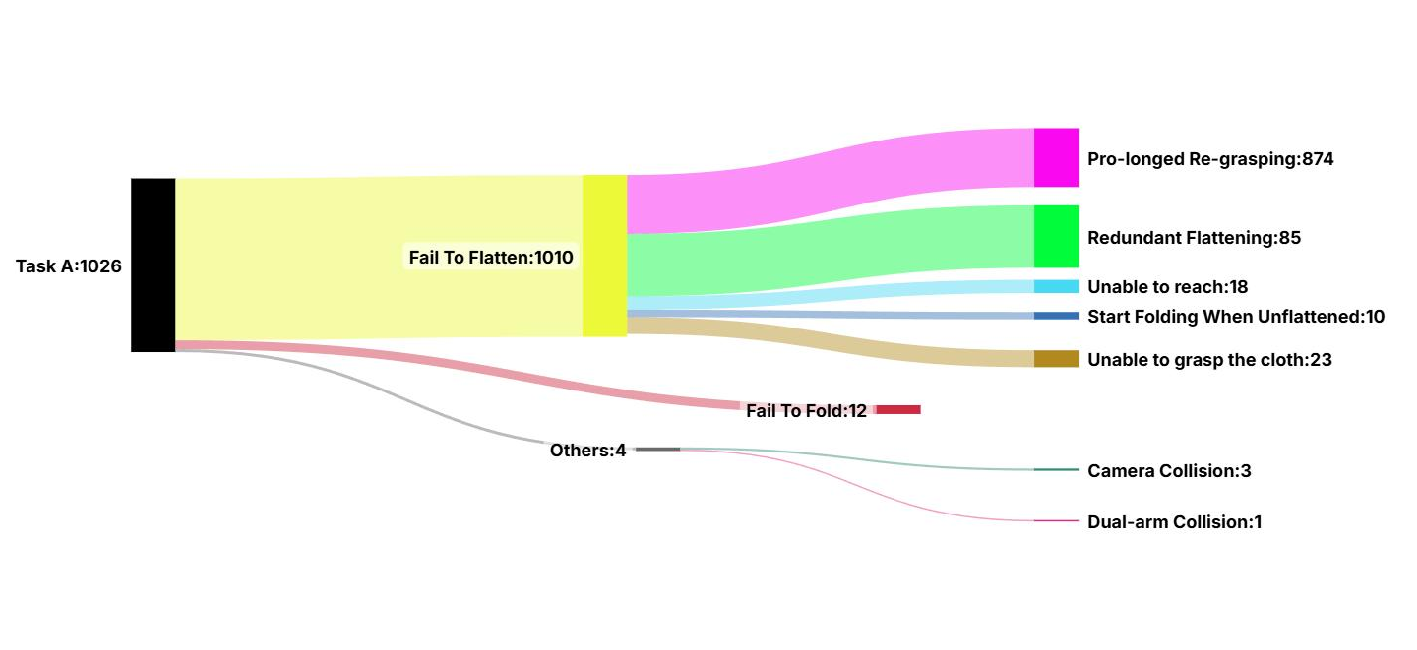
\includegraphics[width=\linewidth]{ch-kai0/images/failure_case_trim.pdf}
  \caption[Failure cases on Task~A]{\textbf{Visualisation of failure cases on Task~A.} Categories of the failure instances recorded during evaluation, with the number of instances in each category.}
  \label{kai0:fig:failure_case}
\end{figure}

\paragraph{Q7. What fundamentally distinguishes different robot foundation models?}
Consistent with the failure modes above, the core distinction lies not in the zero-shot capabilities of the models but in their fine-tuning dynamics, specifically in their plasticity in acquiring new spatial understanding and task-planning skills during post-training. Some architectures, such as $\pi_0$ and $\pi_{0.5}$, show markedly higher adaptability than others, which suggests that their pre-trained weights provide a more robust initialisation for downstream learning. The field therefore needs new metrics that benchmark the intrinsic representational quality of foundation models, rather than relying solely on success rates in simplistic evaluation environments.

%-------------------------------------------------------------------------------
\section{Additional Related Work}\label{kai0:app:related}

\subsection{Reinforcement Learning for Robustness}\label{kai0:app:related_rl}
Reinforcement learning has become a route to post-training VLA policies in simulation~\cite{liu2023libero,mu2025robotwin,mees2022calvin,lu2025vla,li2025simplevla,chen2025tgrpo} and on real robots~\cite{luo2025hilserl,xiao2025PLD,luo2024serl}. Advantage-conditioned approaches~\cite{amin2026pistar06,frans2025diffusion,kumar2019reward} guide generation without differentiating through the full diffusion or flow-matching process~\cite{lei2025rl}. Related methods use vision-language models to score progress~\cite{ma2024gvl,zhang2025rewind,zhai2025vlac,ghasemipour2025self}, form differences $V(s')-V(s)$, and use the resulting signal in policy learning~\cite{amin2026pistar06,wu2023elastic,kuba2023advantage}. The variance of a difference depends on both individual errors and their covariance. Stage Advantage instead predicts relative progress with $f_{\theta}(s,s'\mid g)$ and conditions on stage information to address observational ambiguity. This choice does not produce lower variance or more accurate supervision by construction; those properties require matched empirical evaluation. The source's smoothness measures and downstream task metrics are therefore reported separately.

\subsection{Control Methods}\label{kai0:app:related_control}
Asynchronous inference reduces latency, but existing methods face significant implementation hurdles. SmolVLA~\cite{shukor2025smolvla} employs a naive chunk-switching strategy, which results in severe misalignment between prediction and execution and in unstable control. Similarly, the concurrent A2C2~\cite{sendai2025leave} addresses the misalignment by adding auxiliary correction heads, which necessitates architectural modifications. In contrast, \chiz augments asynchronous inference with temporal chunk-wise smoothing without adding a prediction head. Its total computational overhead is not quantified here.

%-------------------------------------------------------------------------------
\section{Method Details}\label{kai0:app:method}

\subsection{Origin of the Name}\label{kai0:app:name}
The approach is grounded in the principle of \textbf{K}inetics \textbf{A}ligned to \textbf{I}ntelligence. ``Kinetics'' defines the operational domain, spanning training ($P_{\mathrm{train}}$) and deployment ($P_{\mathrm{test}}$), while ``Intelligence'' denotes the inductive bias encoded in the parameter space ($Q_{\mathrm{model}}$). This initial iteration is designated KAI\textsubscript{0}. Noting the phonetic resemblance between ``KAI'' and the Greek letter $\chi$, the system is named \chiz, in tribute to the state-of-the-art $\pi$ series of policies.

\subsection{Model Arithmetic}\label{kai0:app:ma}
The source describes four checkpoints trained on different data subsets. It also describes a \emph{single-best} candidate selected by lowest validation loss and a \emph{full-data} candidate trained on the aggregated data. Its supplementary recipe uses inverse-loss weighting, whereas its main-text discussion favours greedy search. Neither statement identifies unambiguously the recipe that produced the complete-system Task~A result.

The final checkpoint identifiers, common initialisation, subset manifests, seeds, coefficients and stopping rules are unavailable, as is the separation of recovery data used for selection, training and final evaluation. Both candidate strategies are therefore retained in Section~\ref{kai0:sec:ma} as source descriptions; this thesis does not choose one as the verified final method.

\subsection{Stage Advantage}\label{kai0:app:sa}
The source constructs image pairs from the same episode and derives a relative-progress target from their timestamps. Stages correspond to two sub-goals for Task~A (flattening, folding), four for Task~B (retrieving, flattening, folding, handover) and three for Task~C (retrieving, dressing the rack, hanging).

The source gives two incompatible interpretations of its reported $\epsilon=0.3$: an absolute threshold in Eq.~\eqref{kai0:eq:indicator}, and a ranking rule that labels the top 0.3 fraction of samples positive. The latter need not coincide with an advantage threshold of 0.3. The implemented rule, ranking population, tie handling, timestamp normalisation, sampled horizons, stage inputs and policy conditioning are unavailable. The value is retained as an unresolved source report and is not silently converted between interpretations.

\subsection{Train--Deploy Alignment}\label{kai0:app:tda}
Standard DAgger data are collected in three steps.
\begin{enumerate}
  \item The environment is initialised and policy inference starts.
  \item When the policy fails repeatedly, defined as failing to grasp the clothes for more than 10 consecutive attempts or producing repetitive action patterns without progress for more than 10 steps, it is interrupted. On the software side, the policy stops receiving new observations and produces no further actions; on the hardware side, the robot is held in its current state and switched to teleoperation mode to accept human correction.
  \item Both the human correction and the preceding policy rollout are saved.
\end{enumerate}
The source calls its second procedure ``heuristic DAgger'', but it does not run the current policy to reach the queried state. This thesis therefore calls it \emph{targeted recovery demonstration collection}: an operator initialises the system in a manually designed failure state and demonstrates a recovery. The smoothing implementation still requires verification of $d_{\max}$, $m_{\min}$, command timing, buffer initialisation and residual/consumed indexing.

%-------------------------------------------------------------------------------
\section{Experimental Details}\label{kai0:app:exp}

\subsection{Data, Training Strategy and Evaluation Criteria}\label{kai0:app:data}
\begin{itemize}
  \item \textbf{Data scale and diversity.} The source reports collection at 30\,Hz under varied garment states and lighting: 2668 episodes for Task~A (mean 30.41\,s), 3519 for Task~B (34.40\,s) and 2988 for Task~C (39.01\,s), including shorter DAgger interventions. These are recorded-data statistics. Their aggregation, the subsets used for training and selection, and their relation to the separately reported 20-hour-per-task budget remain unverified.
  \item \textbf{Training strategy and hyper-parameters.} The source reports all-parameter flow-matching post-training of $\pi_{0.5}$, independently per task. Table~\ref{kai0:tab:hyperparams} preserves the reported settings. It does not establish whether the step count applies to each of four MA candidates or to a complete pipeline, or provide total compute for model selection and SA fitting.
  \item \textbf{Evaluation criteria (average score).} A rule-based evaluation protocol assigns partial credit for the completion of sub-goals. Table~\ref{kai0:tab:score} lists the sub-goals and their scores.
\end{itemize}
The recorded episode durations imply totals that do not match the separate claim of about 20 hours per task under a simple sum, but the source does not identify which demonstrations, recoveries or validation records belong to that budget. It also reports 8 A100 GPUs without total GPU-hours or whether the training steps apply to each candidate or the full selection pipeline. The chapter therefore treats these as unresolved source descriptions, not as verified resource accounting.
\begin{table}[tb]
  \centering
  \caption[Hyper-parameters for fine-tuning]{Source-reported post-training settings. The 20-hour scope is not reconciled with the episode statistics; total compute and the interpretation of the SA parameter remain to be verified. These are not the costs of pre-training $\pi_{0.5}$.}
  \label{kai0:tab:hyperparams}
  \small
  \setlength{\tabcolsep}{3pt}
  \begin{tabularx}{\linewidth}{@{}>{\raggedright\arraybackslash}X>{\raggedright\arraybackslash}p{4.8cm}@{}}
    \toprule
    \textbf{Hyper-parameter} & \textbf{Value} \\
    \midrule
    \multicolumn{2}{l}{\textit{Data and input}} \\
    Demonstration hours (source claim) & $\sim$20\,h per task; scope unresolved \\
    Action chunk length $K$ & 50 \\
    Execution frequency & 100\,Hz \\
    \midrule
    \multicolumn{2}{l}{\textit{Optimisation}} \\
    Training steps (scope unresolved) & 80{,}000 \\
    Batch size & 128 \\
    Optimiser & AdamW \\
    Learning rate & $2.5 \times 10^{-5}$ \\
    Cosine decay steps & 10{,}000 \\
    Conditioned noise level $\sigma$ & [0.001, 1.0] \\
    Gradient clip & 1.0 \\
    \midrule
    \multicolumn{2}{l}{\textit{Module-specific}} \\
    MA: number of checkpoints & 4 \\
    SA: reported parameter $\epsilon$ & 0.3; interpretation unresolved \\
    \midrule
    \multicolumn{2}{l}{\textit{Infrastructure}} \\
    Training GPUs & 8 $\times$ A100 \\
    Inference GPUs & RTX 4090 \\
    \bottomrule
  \end{tabularx}
\end{table}

\begin{table}[tb]
  \centering
  \caption{Source-reported milestone credits for the average score. Each task branch sums to 100; the correspondence between these credits and the plotted success rates requires the consistency check below.}
  \label{kai0:tab:score}
  \small
  \setlength{\tabcolsep}{3pt}
  \begin{tabularx}{\linewidth}{@{}lXc@{}}
    \toprule
    \textbf{Task} & \textbf{Sub-goal} & \textbf{Score} \\
    \midrule
    \multirow{4}{*}{Task A (easy)}
      & Flatten garment & +40 \\
      & 1st fold & +20 \\
      & 2nd fold & +20 \\
      & 3rd fold & +20 \\
    \midrule
    \multirow{5}{*}{Task B, T-shirt (medium)}
      & Retrieve \& flatten & +40 \\
      & 1st fold & +15 \\
      & 2nd fold & +15 \\
      & 3rd fold & +15 \\
      & Stack to top-left & +15 \\
    \midrule
    \multirow{3}{*}{Task B, shirt (medium)}
      & Retrieve from basket & +30 \\
      & Flatten & +50 \\
      & Pull to right-side table & +20 \\
    \midrule
    \multirow{6}{*}{Task C (hard)}
      & Pull garment rightward & +15 \\
      & Grasp collar & +15 \\
      & Grasp hanger & +15 \\
      & Insert hanger into sleeve & +20 \\
      & Hook left collar on hanger & +20 \\
      & Hang on standing rack & +15 \\
    \bottomrule
  \end{tabularx}
\end{table}
\paragraph{Pending success--score consistency check.}\label{kai0:app:scorecheck}
If a successful trial receives all milestone credits in Table~\ref{kai0:tab:score}, partial credits are nonnegative, and success rate and score use the same trials and weights, the average score cannot be below the success percentage. In Fig.~\ref{kai0:fig:app_soup_b}, however, the full-data panels and the in-domain inverse-loss panels show score bars below their success-rate bars by more than visual reading uncertainty. A similar discrepancy appears in a Task~B control setting in Fig.~\ref{kai0:fig:app_tda_b_abs}. This is a conditional consistency problem in the reported metrics, not an inference of misconduct or a determination of which plotted value is wrong.

The original figures are retained unchanged as source records. The affected panels are not used to support cross-metric superiority or aggregate-improvement claims. Per-trial success and milestone records, sample weights, configuration identifiers and plotting code are unavailable, so the discrepancy cannot be resolved here. Any future correction must follow those records rather than approximate readings of the figures.
\subsection{Hardware Configuration and Inference Details}\label{kai0:app:hardware}
As illustrated in Fig.~\ref{kai0:fig:robot_setup}, the experimental setup includes two bimanual systems: one built from AgileX Robotics Piper arms and the other from ARX Robotics X5 arms. Both dual-arm platforms have two 6-DoF arms equipped with 1-DoF parallel grippers. A key kinematic difference lies in the configuration of the fifth joint, which is a pitch joint on the AgileX Piper arm and a yaw joint on the ARX X5. For perception, each system is equipped with three Intel RealSense D435i cameras (one fixed head view and two wrist views) that capture $640 \times 480$ RGB images. The visual sampling rate is synchronised at 30\,Hz for both data collection and inference, while the low-level joint controllers operate at a higher frequency of 100--200\,Hz. All inference is performed on an Ubuntu 20.04 workstation equipped with an NVIDIA RTX 4090 GPU.

\subsection{Empirical Loss Curve}\label{kai0:app:loss}
Figure~\ref{kai0:fig:loss_curve_sa} retains the source's training loss curves. SA reaches a lower displayed loss, but the target definitions, conditioning and loss normalisation must be comparable before this is evidence of better training. The curves alone do not establish generalisation, progress accuracy or numerical stability; their exact training extent is not resolved by Table~\ref{kai0:tab:hyperparams}.

\begin{figure}[tb]
  \centering
  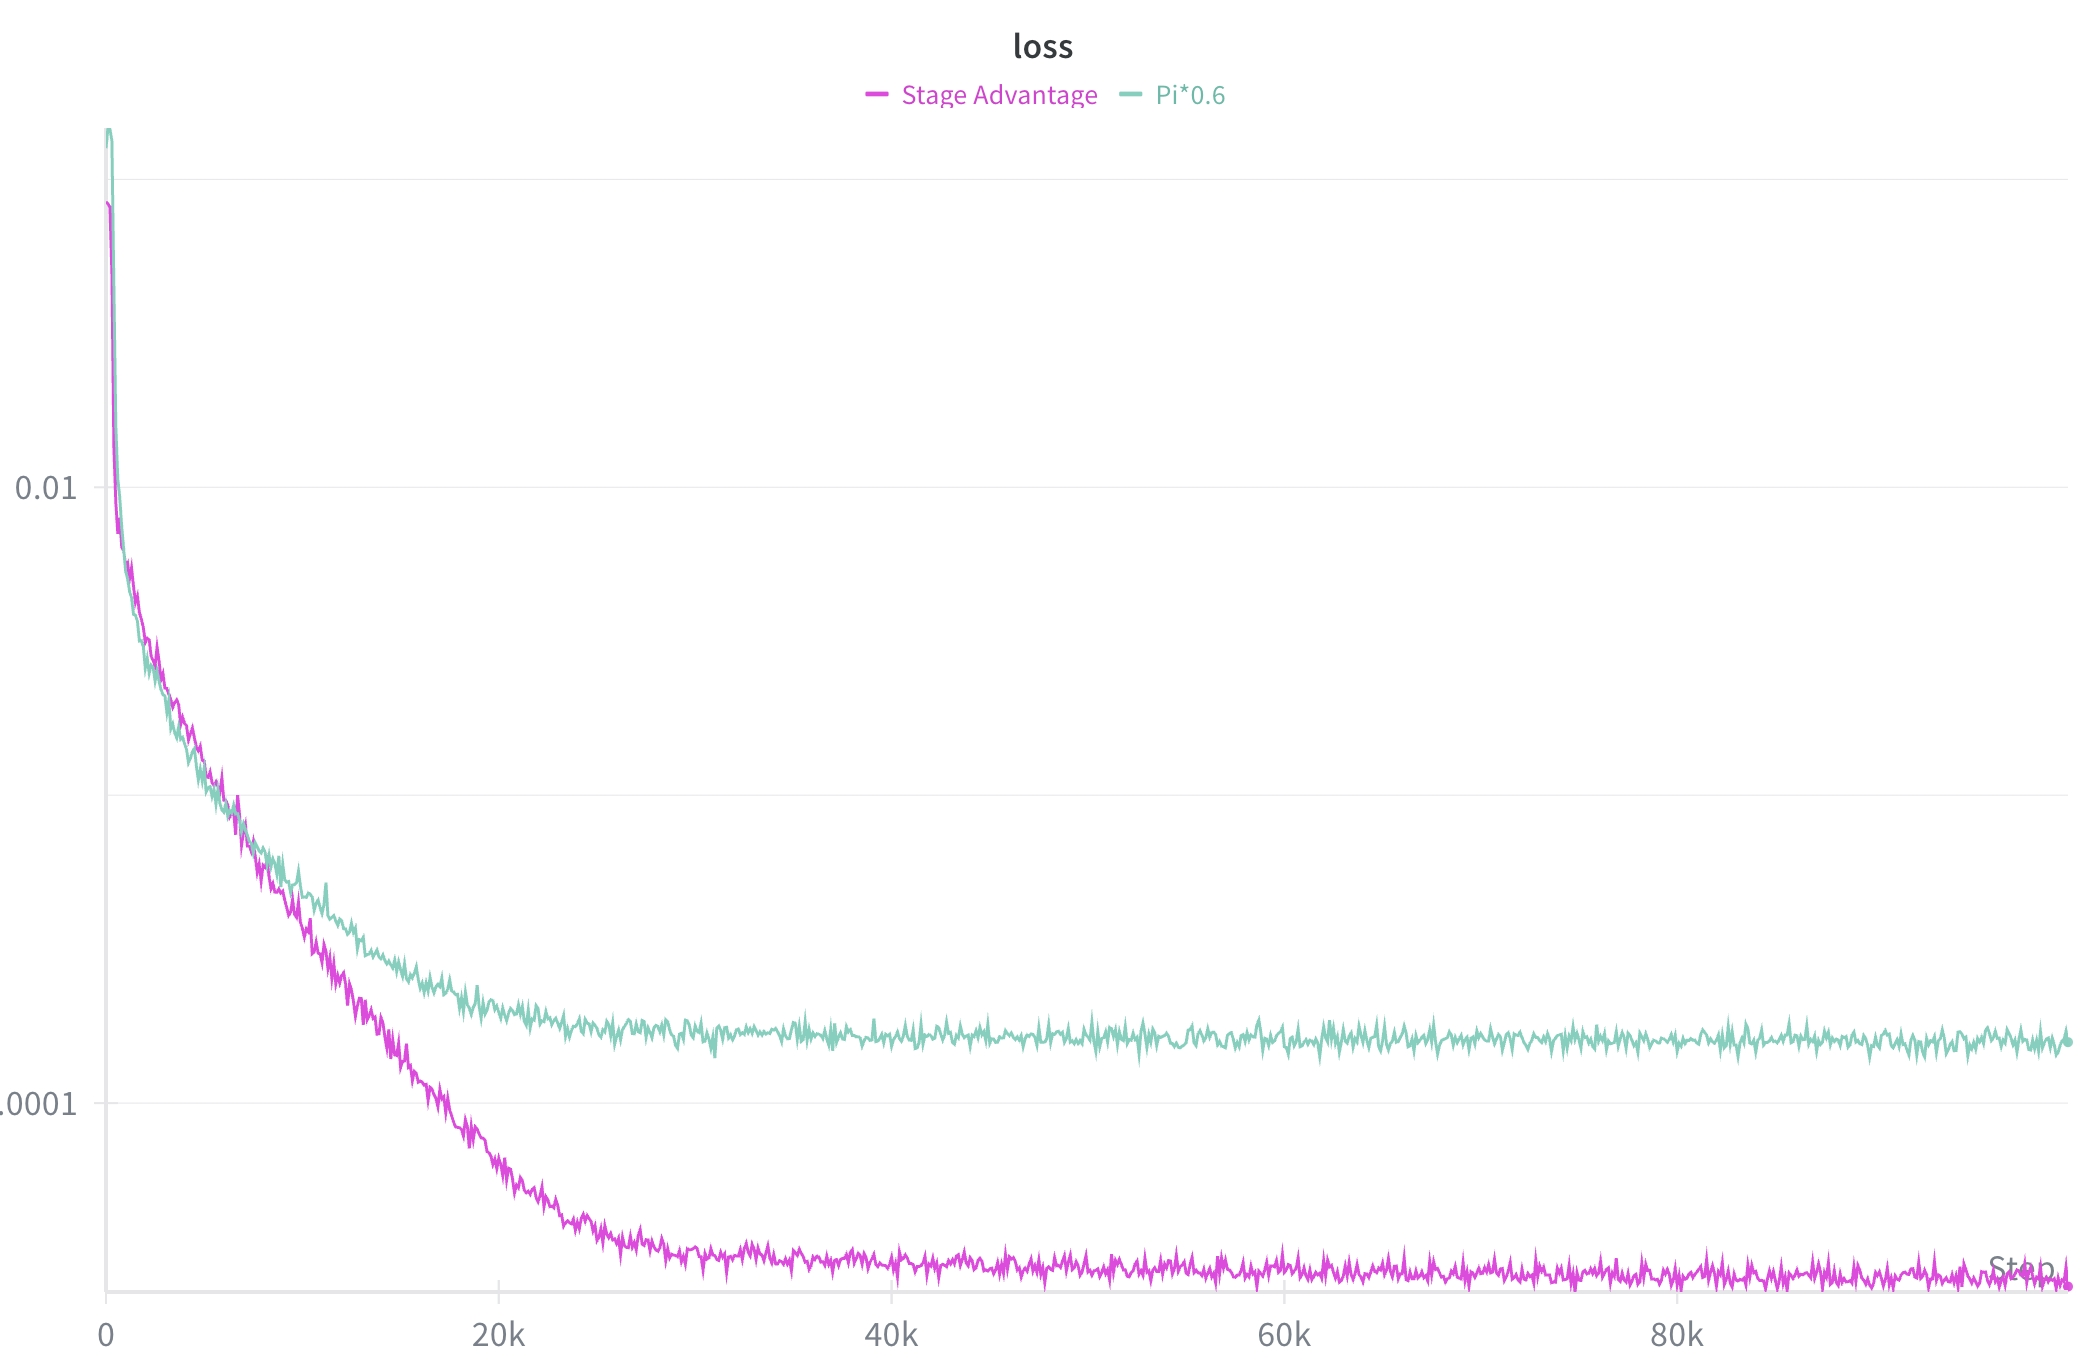
\includegraphics[width=0.65\linewidth]{ch-kai0/images/loss_curve_SA.jpeg}
  \caption[Training loss curves of Stage Advantage and the $\pi^{*}_{0.6}$-style baseline]{\textbf{Source-reported training loss curves.} SA reaches a lower plotted loss than the $\pi^{*}_{0.6}$-style implementation. Different target definitions and conditioning limit cross-method interpretation; the curves alone do not prove accuracy or stability.}
  \label{kai0:fig:loss_curve_sa}
\end{figure}

%-------------------------------------------------------------------------------
\section{Additional Ablations}\label{kai0:app:ablation}

\subsection{Model Arithmetic on Tasks A and B}\label{kai0:app:ablation_ma}
Figure~\ref{kai0:fig:app_soup} preserves the MA comparisons for Tasks~A and~B. In Task~A, merging and OOD selection have metric-dependent effects rather than a uniform advantage. The Task~B success-rate/score panels require the consistency check in Section~\ref{kai0:app:scorecheck}; this draft does not use them to establish cross-metric superiority. More generally, selection by recovery validation loss is a heuristic whose utility depends on the selection data. The plots do not isolate data quality as the cause of variation.

\begin{figure}[tbp]
  \centering
  \begin{subfigure}[t]{0.95\linewidth}
    \centering
    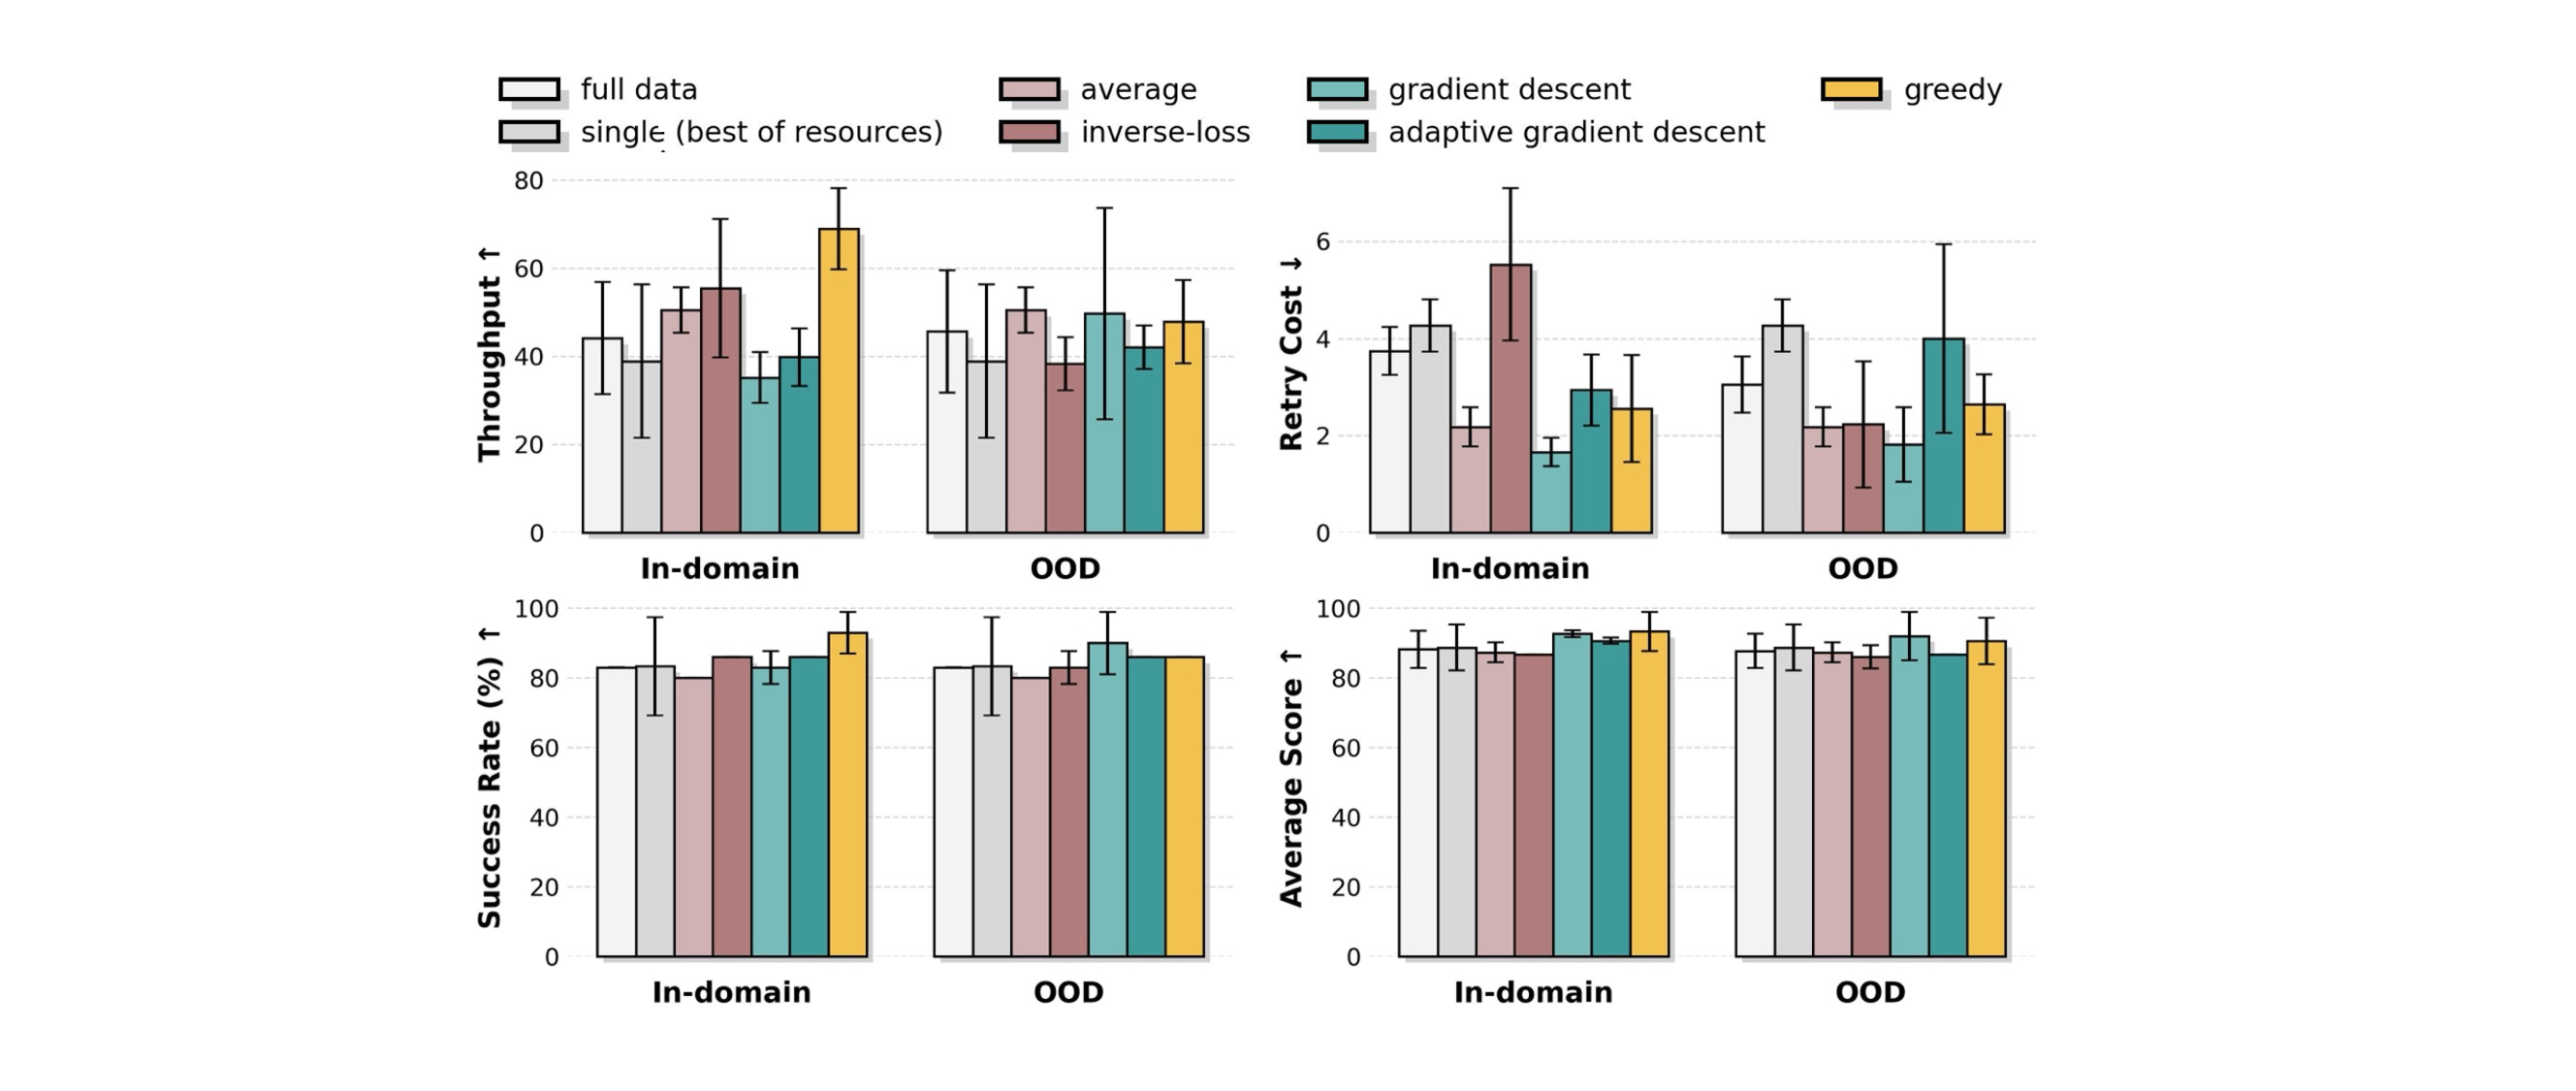
\includegraphics[width=\linewidth]{ch-kai0/images/souping_ff_compress.pdf}
    \caption{Model Arithmetic on Task~A}
    \label{kai0:fig:app_soup_a}
  \end{subfigure}

  \medskip
  \begin{subfigure}[t]{0.95\linewidth}
    \centering
    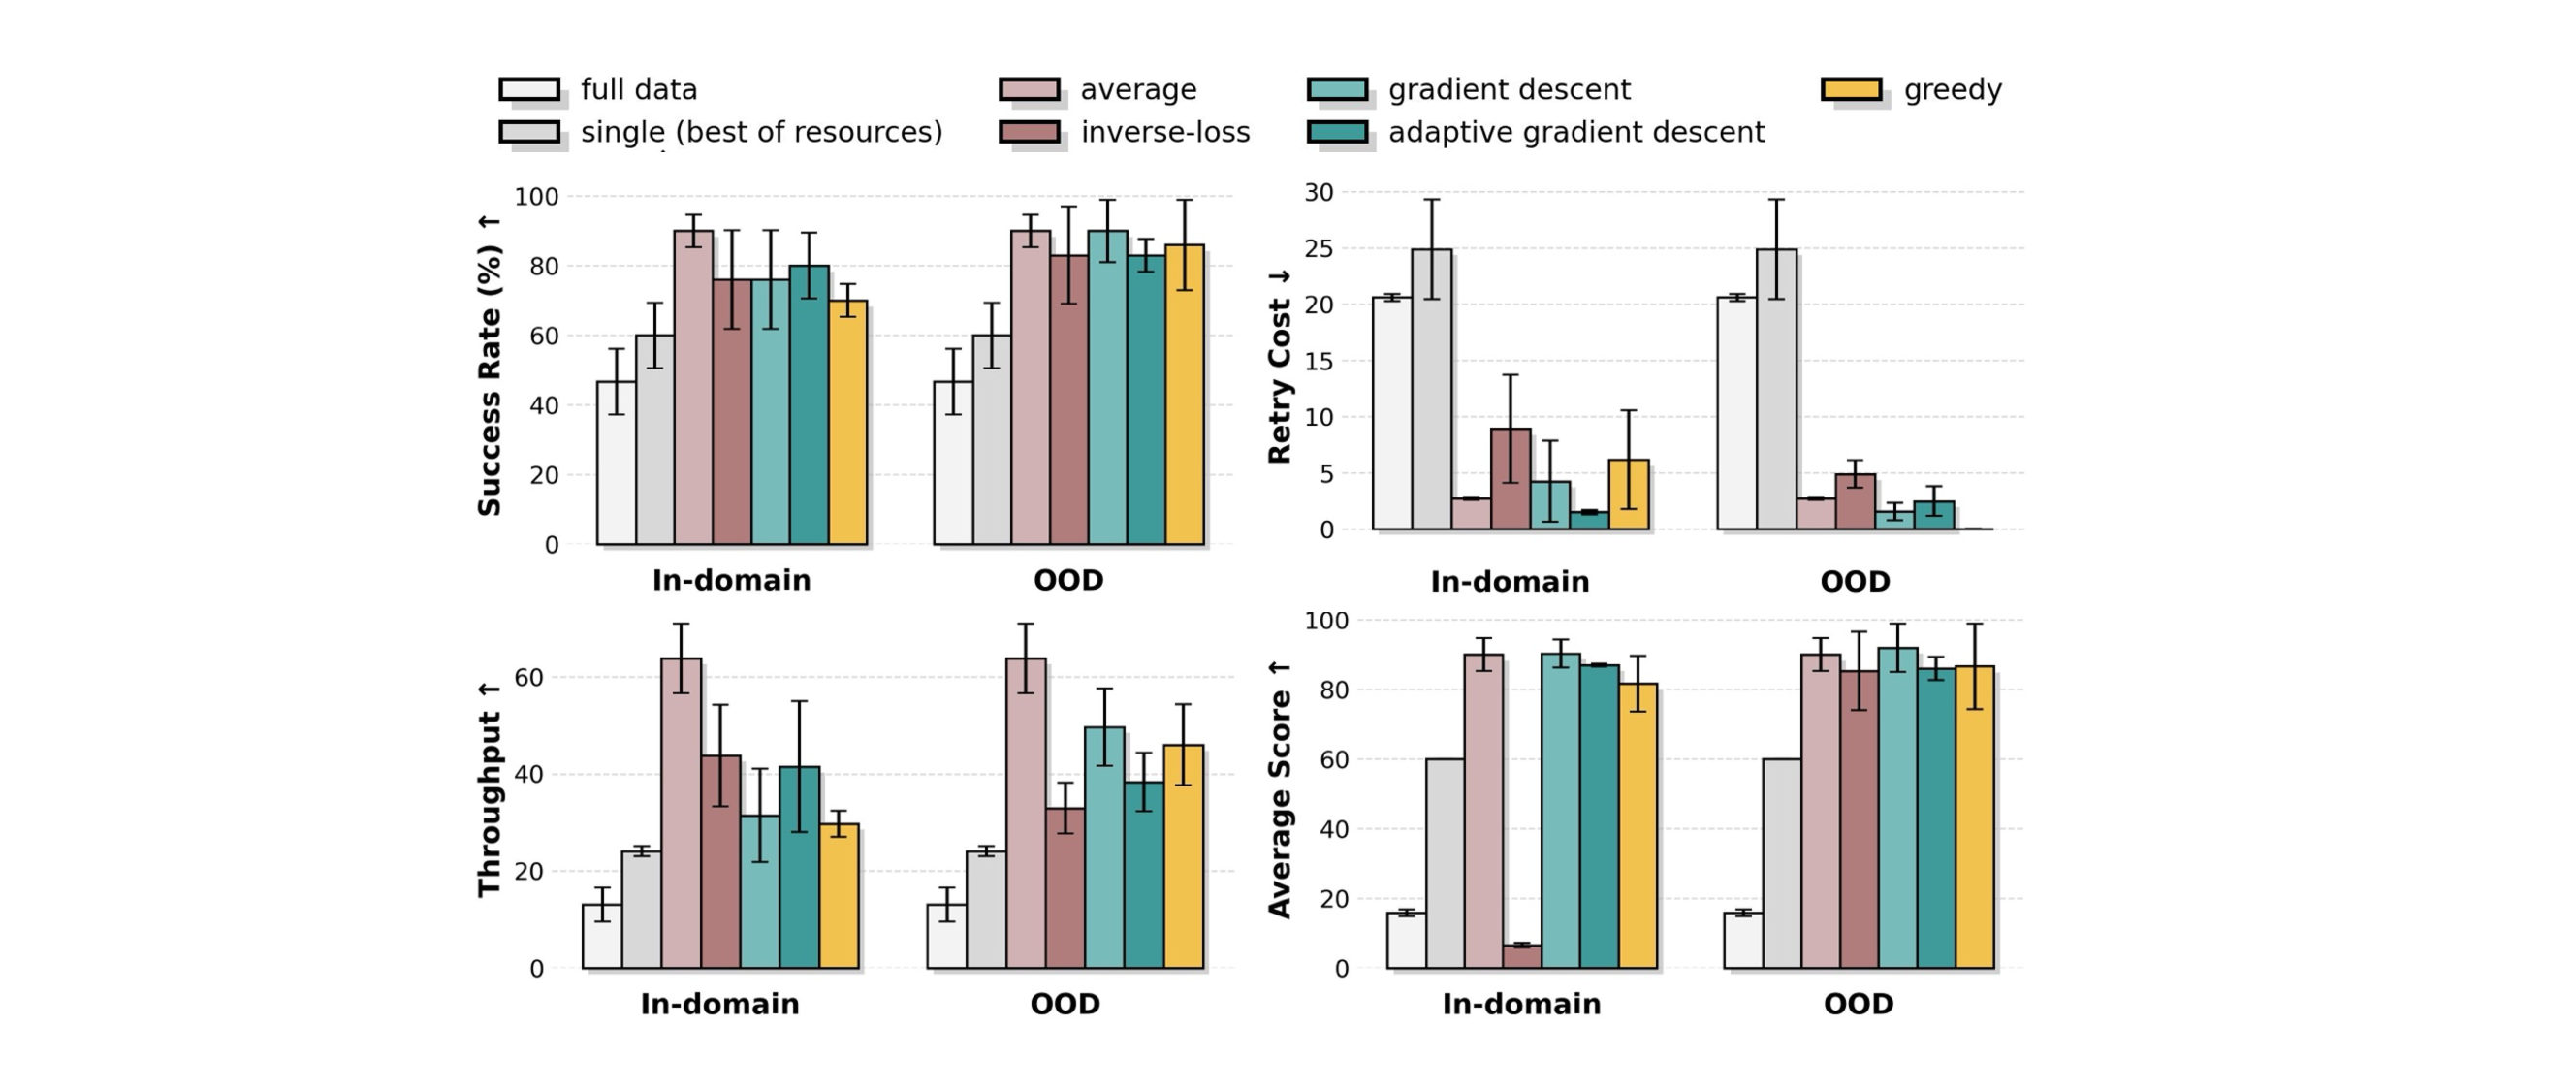
\includegraphics[width=\linewidth]{ch-kai0/images/souping_demoA_compress.pdf}
    \caption{Model Arithmetic on Task~B}
    \label{kai0:fig:app_soup_b}
  \end{subfigure}
  \caption[Ablation of Model Arithmetic on Tasks~A and~B]{\textbf{Source-reported Model Arithmetic comparisons.} The original Task~A and Task~B plots are retained. Task~A shows metric-dependent trade-offs. Task~B's success-rate and score panels are pending verification and are not used for cross-metric conclusions (Section~\ref{kai0:app:scorecheck}).}
  \label{kai0:fig:app_soup}
\end{figure}

\subsection{Stage Advantage on Task C}\label{kai0:app:ablation_sa}
Figure~\ref{kai0:fig:app_sa_c} preserves the Task~C ablation. Direct+Stage has smoother reported signals but lower plotted success rate, throughput and average score than the value-difference baseline. Reduced retry cost can coexist with failure, so it does not reverse that interpretation. The results do not identify whether missing pre-training priors, the progress proxy or another implementation factor causes this pattern.

\begin{figure}[tb]
  \centering
  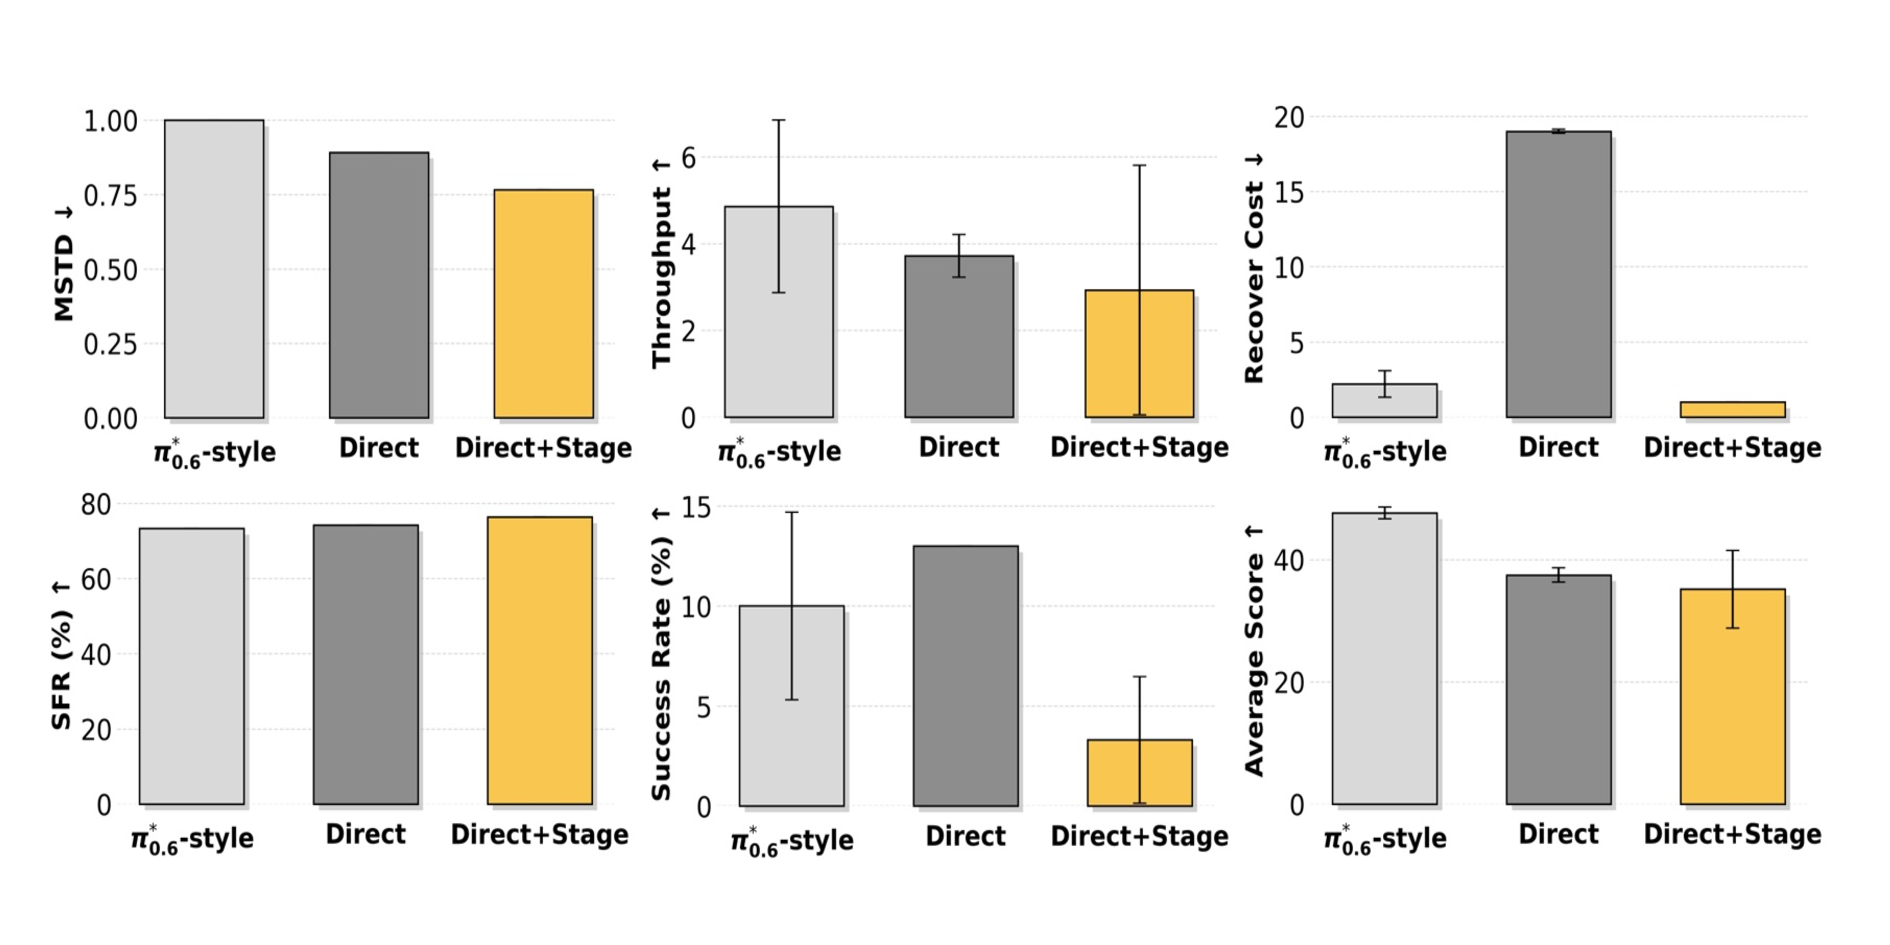
\includegraphics[width=0.85\linewidth]{ch-kai0/images/advantage_demoB_compress.pdf}
  \caption[Ablation of Stage Advantage on Task~C]{\textbf{Stage Advantage on Task~C.} The source reports lower MSTD and higher SFR for Direct+Stage, but lower success rate, throughput and average score than the value-difference baseline. The smoothness definitions remain to be checked. ``Recover Cost'' denotes the source's retry cost.}
  \label{kai0:fig:app_sa_c}
\end{figure}

\subsection{Train--Deploy Alignment on All Tasks}\label{kai0:app:ablation_tda}
Figures~\ref{kai0:fig:app_tda_a}--\ref{kai0:fig:app_tda_c} preserve the comparisons of absolute and delta joint actions with augmentation and control strategies. Their effects vary with task and endpoint; they do not establish that smoothing or its combination with RTC is uniformly preferable. Task~C appears sensitive to action parameterisation, but the proposed explanation in terms of hanger-insertion precision is not isolated by these ablations. The Task~B success/score discrepancy noted in Section~\ref{kai0:app:scorecheck} also limits cross-metric interpretation of its control plots.

\begin{figure}[tbp]
  \centering
  \begin{subfigure}[t]{0.8\linewidth}
    \centering
    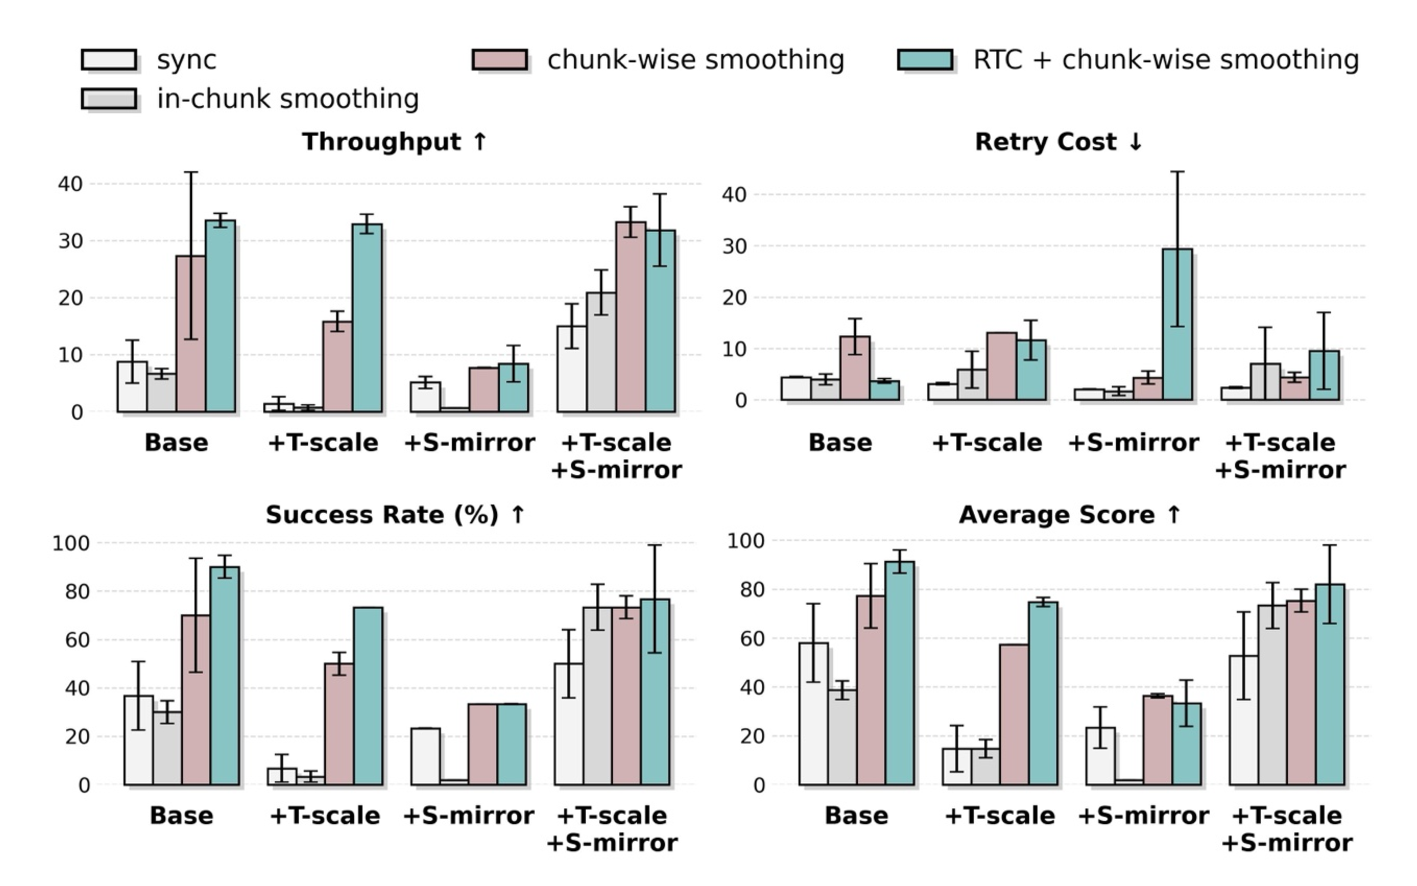
\includegraphics[width=\linewidth]{ch-kai0/images/ff_abs_compress.pdf}
    \caption{Absolute joint}
    \label{kai0:fig:app_tda_a_abs}
  \end{subfigure}

  \medskip
  \begin{subfigure}[t]{0.8\linewidth}
    \centering
    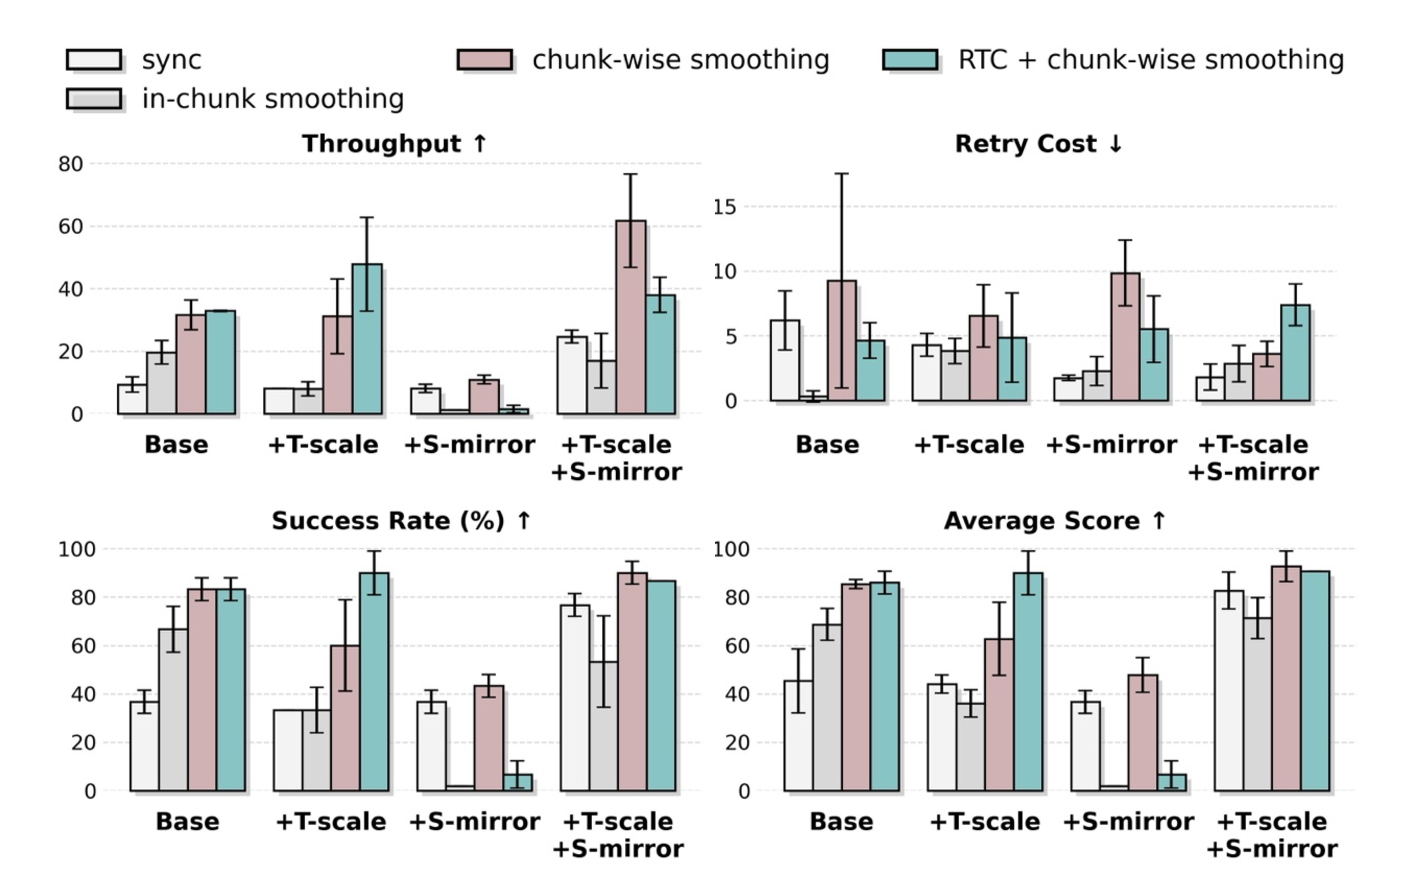
\includegraphics[width=\linewidth]{ch-kai0/images/ff_delta_compress.pdf}
    \caption{Delta joint}
    \label{kai0:fig:app_tda_a_delta}
  \end{subfigure}
  \caption[Control strategies and augmentation on Task~A with two action representations]{\textbf{Task~A control and augmentation comparisons.} Absolute (a) and delta (b) joint actions show setting-dependent trade-offs. Smoothing and its combination with RTC improve some reported outcomes, not every endpoint or augmentation setting.}
  \label{kai0:fig:app_tda_a}
\end{figure}

\begin{figure}[tbp]
  \centering
  \begin{subfigure}[t]{0.8\linewidth}
    \centering
    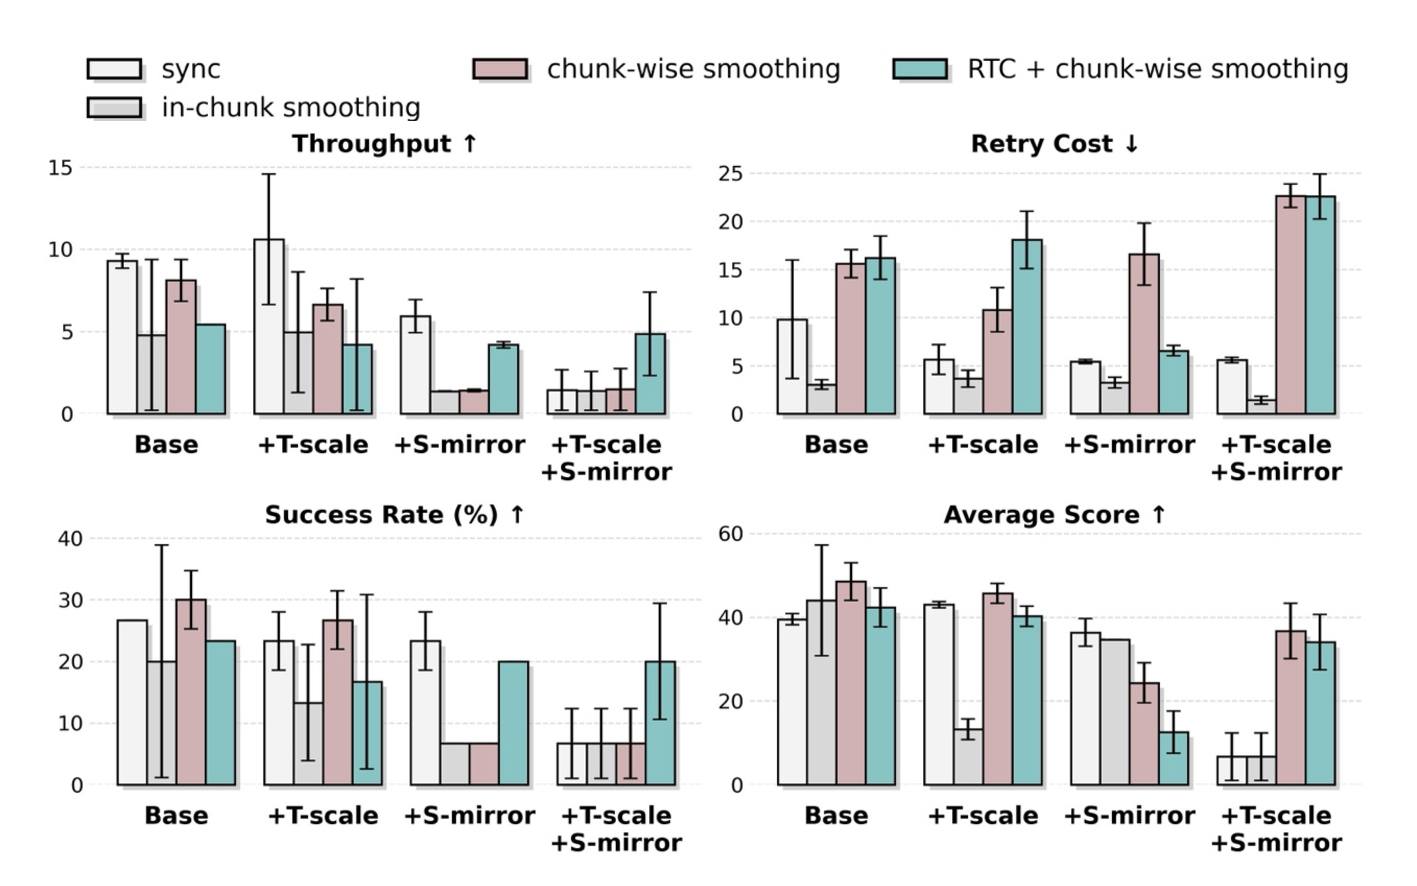
\includegraphics[width=\linewidth]{ch-kai0/images/demoA_abs_compress.pdf}
    \caption{Absolute joint}
    \label{kai0:fig:app_tda_b_abs}
  \end{subfigure}

  \medskip
  \begin{subfigure}[t]{0.8\linewidth}
    \centering
    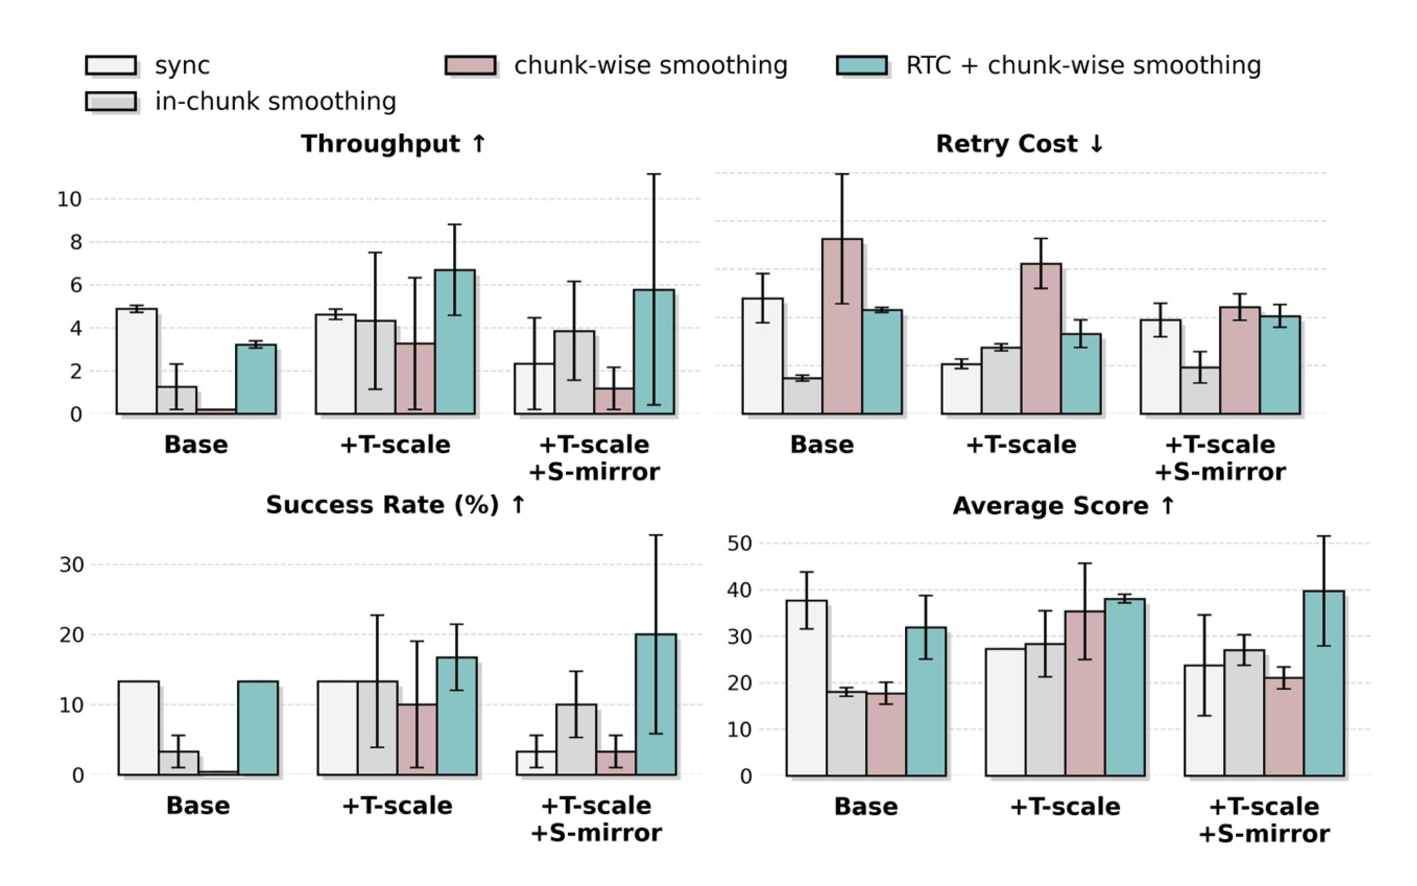
\includegraphics[width=\linewidth]{ch-kai0/images/demoA_delta_compress.pdf}
    \caption{Delta joint}
    \label{kai0:fig:app_tda_b_delta}
  \end{subfigure}
  \caption[Control strategies and augmentation on Task~B with two action representations]{\textbf{Source-reported Task~B control and augmentation comparisons.} Effects depend on action representation and augmentation. The success-rate/score consistency check in Section~\ref{kai0:app:scorecheck} must be resolved before the affected panels support cross-metric superiority claims.}
  \label{kai0:fig:app_tda_b}
\end{figure}

\begin{figure}[tbp]
  \centering
  \begin{subfigure}[t]{0.8\linewidth}
    \centering
    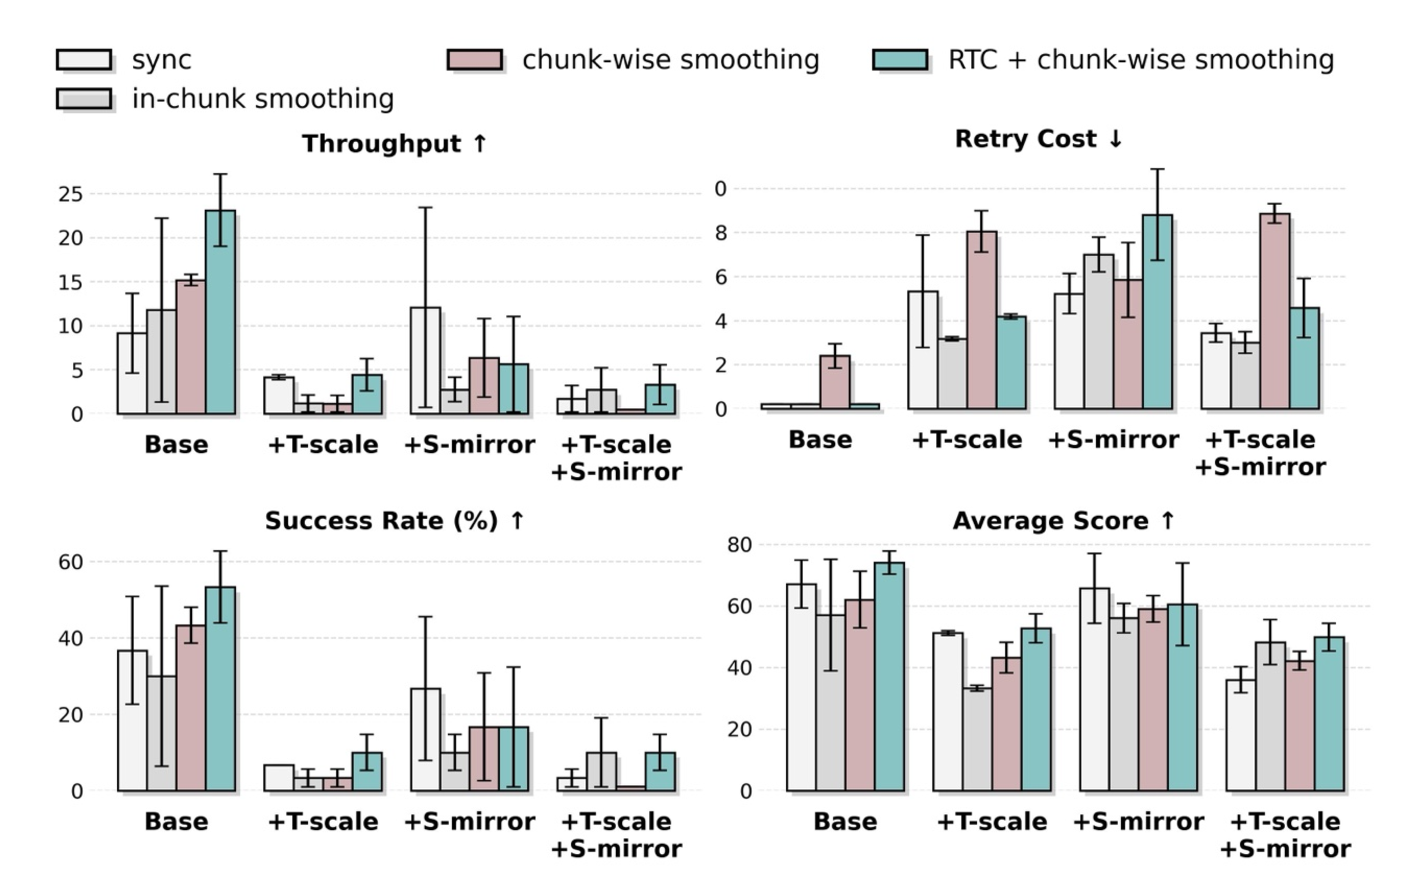
\includegraphics[width=\linewidth]{ch-kai0/images/demoB_abs_compress.pdf}
    \caption{Absolute joint}
    \label{kai0:fig:app_tda_c_abs}
  \end{subfigure}

  \medskip
  \begin{subfigure}[t]{0.8\linewidth}
    \centering
    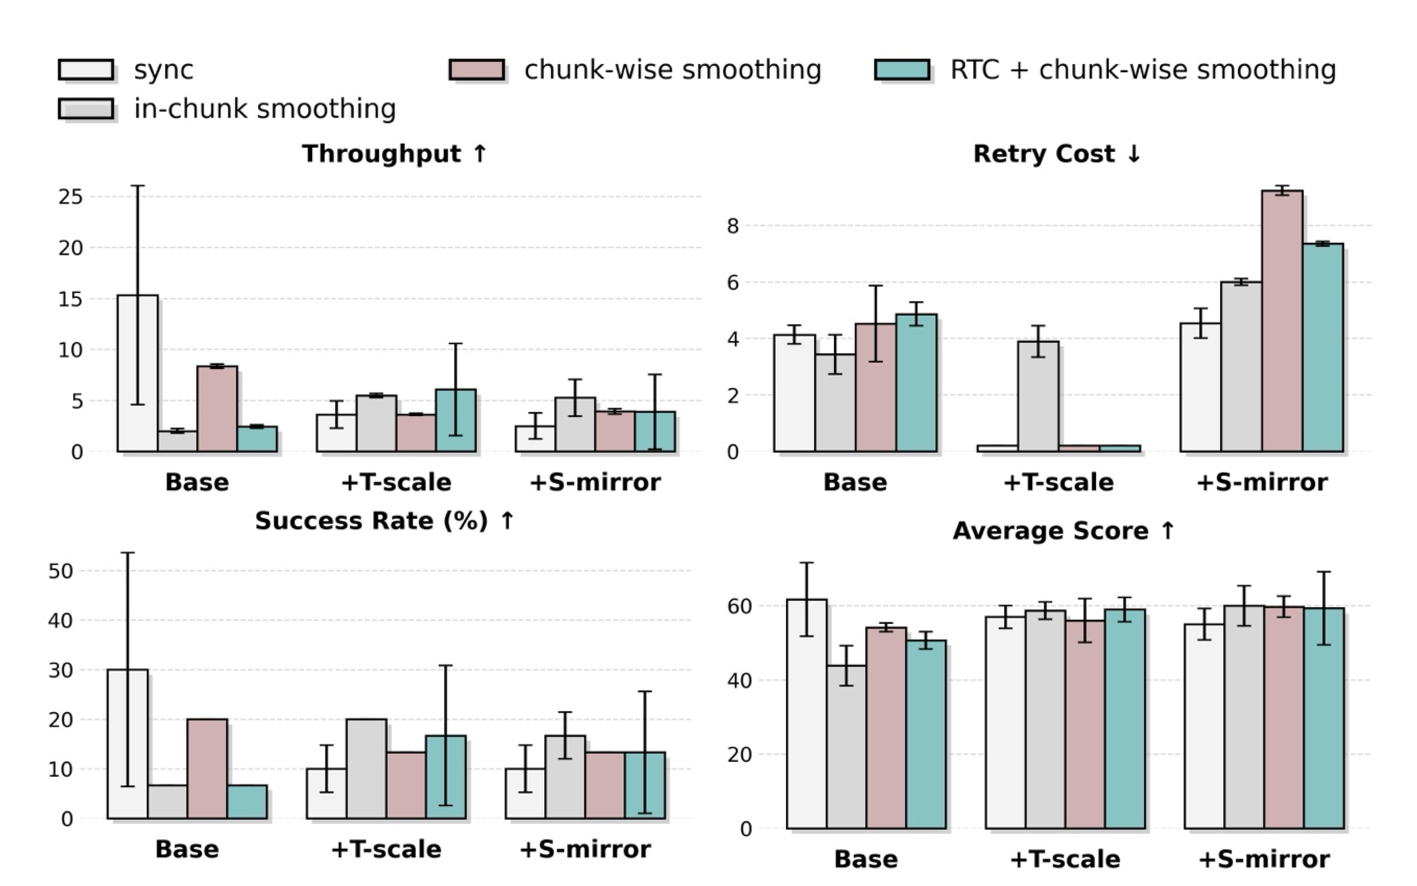
\includegraphics[width=\linewidth]{ch-kai0/images/demoB_delta_compress.pdf}
    \caption{Delta joint}
    \label{kai0:fig:app_tda_c_delta}
  \end{subfigure}
  \caption[Control strategies and augmentation on Task~C with two action representations]{\textbf{Ablation of control strategies and spatio-temporal augmentation on Task~C with different action representations.} Because Task~C is a fine-grained task, the overall success rate is relatively low with both absolute and delta joint control, and the results are sensitive to the choice of action representation.}
  \label{kai0:fig:app_tda_c}
\end{figure}

%-------------------------------------------------------------------------------
\section{Failure Case Analysis}\label{kai0:app:failure}
The source categorises 1026 failure instances during Task~A evaluation, of which 1010 are assigned to flattening (Fig.~\ref{kai0:fig:failure_case}). These counts are retained, but their mapping to configurations, trials and retries and the repeated-event counting rules are not specified. They are not treated as independent failed episodes or a population failure rate. The distribution motivates attention to flattening recovery without by itself establishing the causal effectiveness of DAgger.

%-------------------------------------------------------------------------------
\section{Data and Code Release}\label{kai0:app:license}
The code, data and model weights of \chiz are released to facilitate research in the community. The data are released under the CC BY-NC-SA 4.0 licence and the code under the Apache-2.0 licence; the code is available at \url{https://github.com/OpenDriveLab/KAI0}. Linking each reported result to the exact code version, configuration and checkpoint remains part of the verification in Sections~\ref{kai0:app:ma}--\ref{kai0:app:data}.
